%Procedures
\section{Procedures}
\label{af:p}

\subsection{Arc Flash Study Procedures}
\label{af:p:afsp}

\emph{CSA Z462} focuses on safety and the way in which a worker plans and executes a task. When it's necessary to work on energized equipment, written work permits that include a description of the work to be done and the safety hazards involved should be issued. However, wearing the proper safety equipment for the risk hazard involved doesn't guarantee that a worker will remain free from injury or burns. Its purpose is to reduce deaths and life threatening burns.\\

The focus of \emph{IEEE Std. 1584} is the radiated heat or incident energy produced by an arcing fault that falls on a given surface. A bolted fault doesn't produce any radiated flash energy since no arc is involved. A value of 1.2 calorie/cm2 (1.2 calorie/cm2=5.02 Joules/cm2=5.02 Watt-sec/cm2) for a clearing time of 0.1 second is the incident energy level generally used as a guide to restrict the flash hazard to a second-degree or curable burn. In order to maintain that same level of injury, if the clearing time were increased to 1.0 second, the energy level would have to be reduced to 0.12 calorie/cm2.\\

To properly estimate the exposure hazard, it's necessary to have the maximum bolted short-circuit current, the arcing fault current, and the operating time of the interrupting device at the arcing fault current. The incident energy should be calculated at maximum and at 85\% of maximum arc fault current levels. Due to the inverse nature of protective devices, such as fuses and relays, a longer operating time at lower arcing currents can result in a higher energy exposure.\\

To model the power distribution system effectively, and to obtain as accurate results as possible, a number of parameter / factors have to be determined:\\ 

\noindent\textbf{Equipment Class } \\
\noindent Classes of equipment included in IEEE 1584 and typical bus gaps are shown in table below: 

\begin{center}
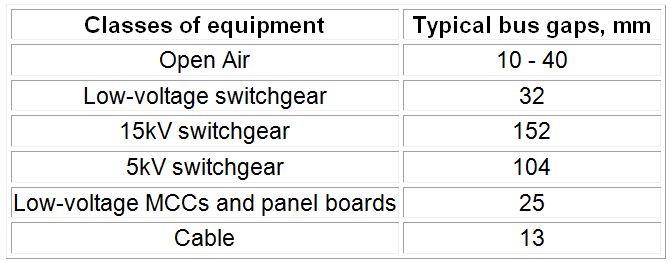
\includegraphics[width=5in, keepaspectratio=true]{Images/Gaps.png} \\
\end{center}

\noindent\textbf{Gap between Conductors } \\  
\noindent Equipment bus gap in mm. Gaps of 3 to 40 mm are used for low voltage testing to simulate gaps between conductors in low voltage equipment and cables. Gaps 13, 104 and 152 mm. are used in 5 and 15kV equipment testing.\\
   
\noindent\textbf{Grounding Type}    \\
\noindent Two grounding classes are applied in the IEEE 1584 procedure, as follows:
\begin{enumerate}
	\item Ungrounded, this included ungrounded, high-resistance grounding and low-resistance grounding.
	\item Solidly grounded. 
\end{enumerate}

\noindent\textbf{Working Distance }  \\ 
\noindent Typical working distance is the sum of the distance between the workers standing in front of the equipment, and from the front of the equipment to the potential arc source inside the equipment. \\

\noindent Arc-flash protection is always based on the incident energy level on the person's face and body at the working distance, not the incident energy on the hands or arms. The degree of injury in a burn depends on the percentage of a person's skin that is burned. The head and body are a large percentage of total skin surface area and injury to these areas is much more life threatening than burns on the extremities. \\

\noindent Typical working distances are shown in table below:
\begin{center}
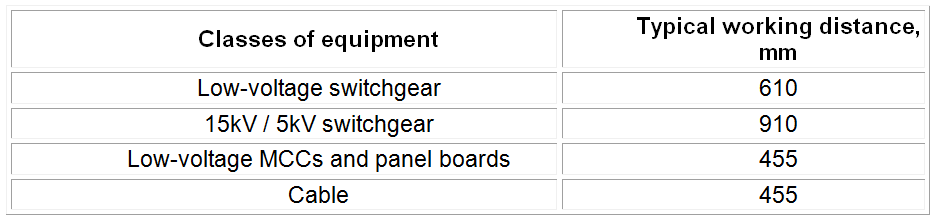
\includegraphics[width=5in, keepaspectratio=true]{Images/WorkingDistance.png} \\
\end{center}

\noindent\textbf{Arc Duration / Total Clearing Time   } \\
\noindent Protective device characteristics, which can be found in the manufacturers, supplied data. For fuses, the manufacturer's time-current curves may include both melting and clearing time. In such a case, the clearing time is used. If they show only the average melt time, 15\% is added to that time, up to 0.03 seconds, and 10\% above 0.03 seconds to determine total clearing time. If the arcing fault current is above the total clearing time at the bottom of the curve (0.01 seconds), 0.01 seconds is used for the time. \\
For circuit breakers with integral trip units, the manufacturer's time-current curves include both tripping time and clearing time. \\

\noindent For relay operated circuit breakers, the relay curves show only the relay operating time in the time-delay region. For relays operating in their instantaneous region, 16 milliseconds are typically allowed on 60 Hz systems for operation. The circuit breaker opening time must be added. Opening times for particular circuit breakers can be verified by consulting the manufacturer's literature. \\
 
  
\noindent\textbf{Available 3 Phase Bolted Fault Current}  \\ 
Available 3 phase bolted fault current for each specific location as determined by the Short Circuit Analysis. \\
 
\noindent\emph{NOTE: Effect of arc current variation on determination of clearing time:    
For protective devices operating in the steep portion of their time-current curves, a small change in current causes a big change in operating time. Incident energy is linear with time, so arc current variation may have a big effect on incident energy. The solution is to make two arc current and energy calculations; one using the calculated expected arc current and one using a reduced arc current that is 15\% lower.}\\ 
